\documentclass[journal,twoside,web]{ieeecolor}
% \documentclass[12pt,peerreview,draftversion,onecolumn,print]{ieeecolor}
\input{preamble.tex}
\usepackage{generic}

% Not sure if needed
\def\BibTeX{{\rm B\kern-.05em{\sc i\kern-.025em b}\kern-.08em
    T\kern-.1667em\lower.7ex\hbox{E}\kern-.125emX}}

\markboth{\journalname, VOL. XX, NO. XX, February 2023}
{Satici: Estimation of the Mass and Damping of a Second-Order Linear System
(February 2023)}

\begin{document}

\title{Estimation of the Mass and Damping of a Second-Order Linear System} 
\author{
    Aykut C. Satici, \IEEEmembership{Member, IEEE}
    \thanks{Not submitted for review in February 2023.}
    \thanks{A. C. Satici is with the Mechanical and Biomedical Engineering Department, Boise State University, Boise, ID 83706 USA
    (e-mail: aykutsatici@boisestate.edu).}
}
\maketitle
% \IEEEpeerreviewmaketitle

  
\begin{abstract} % Abstract of not more than 200 words.
We study the estimation of the mass and the damping of a second-order linear ODE
system using an adaptation law.
\end{abstract}

\begin{IEEEkeywords}
    Adaptive control, estimation
\end{IEEEkeywords}

\section{Introduction}
\label{sec:intro}

We provide a Lyapunov analysis~\cite{khalil2015nonlinear} to prove that our
adaptation law will stabilize the system to a reference trajectory while the
estimates of the mass and the damping tend to their correct values.

\section{Analysis} 
\label{sec:analysis}

We have a linear translational mechanical system with viscous damping, whose
motion is governed by the ODE
%
\begin{equation}
    m \ddot{x} + b\dot{x} = u(x, \dot{x}),
    \label{eq:eom}
\end{equation}
%
where $u(x, \dot{x})$ is a control input that is to be determined for tracking. We are
uncertain of the true values $m$ and $b$ so we denote our guesses for them
by $\hat{m}$ and $\hat{b}$, respectively. Let us introduce the errors in $x$,
$m$ and $b$ to be \[ \tilde{x} = x - x_r, \quad \tilde{m} = m - \hat{m}, \quad
\tilde{b} = b - \hat{b}, \] where $x_r$ is a reference signal for the motion of
the mechanical system. We will postulate update rules for $\hat{m}$ and
$\hat{b}$ and a control law for the mechanical system~\eqref{eq:eom}. The
combined system has the dynamics
%
\begin{align}
    \begin{split}
    m\ddot{\tilde{x}} &= u(x, \dot{x}) - m\ddot{x}_r - b(\dot{x}_r + \dot{\tilde{x}}) \\
    \dot{\hat{m}} &= f(x, \dot{x}) \Rightarrow \dot{\tilde{m}} = -f(x, \dot{x}) \\
    \dot{\hat{b}} &= g(x, \dot{x}) \Rightarrow \dot{\tilde{b}} = -g(x, \dot{x})
    \end{split}
    \label{eq:combined}
\end{align}
%
Let us finally introduce the auxiliary variable $r := \dot{\tilde{x}} + \lambda
\tilde{x}$, where $\lambda > 0$ is a constant whose value is to be determined.
Its dynamics is therefore given by \[ m\dot{r} = m\left(\ddot{\tilde{x}} +
\lambda \dot{\tilde{x}}\right) = u - m(\ddot{x}_r - \lambda\dot{\tilde{x}}) - 
b(\dot{x}_r + \dot{\tilde{x}}). \]

Consider the Lyapunov function candidate
%
\begin{equation}
    V(\tilde{x}, \dot{\tilde{x}}, \tilde{m}, \tilde{b}) = \frac{1}{2}mr^2 + 
    k\lambda\tilde{x}^2 + \frac{1}{2}\tilde{m}^2 + \frac{1}{2}\tilde{b}^2,
    \label{eq:lyap_cand}
\end{equation}
%
where $k$ is another constant to be determined. This is a positive definite
function over the space of $(\tilde{x}, \dot{\tilde{x}}, \tilde{m}, \tilde{b})$.
We take the time derivative of the Lyapunov function candidate and substitute
from the system dynamics. We suppress its functional dependence for brevity.
%
\begin{align*}
    \dot{V} &= r\dot{r} + 2k\lambda\tilde{x}\dot{\tilde{x}} +
    \tilde{m}\dot{\tilde{m}} + \tilde{b}\dot{\tilde{b}}, \\
    &= r\left(u - m\left(\ddot{x}_r - \lambda\dot{\tilde{x}}\right)
    -b\left(\dot{x}_r + \dot{\tilde{x}} \right)\right) +
    2k\lambda\tilde{x}\dot{\tilde{x}} \\ &\phantom{1234}- \tilde{m}f - \tilde{b}g.
\end{align*}
%
This expression informs the selection of the control law as \[ \boxed{u(x, 
\dot{x}) = \hat{m}\left(\ddot{x}_r - \lambda\dot{\tilde{x}}\right) +
\hat{b}\left(\dot{x}_r + \dot{\tilde{x}}\right) - kr}. \] Substituting this
controller into the expression for $\dot{V}$ gives
%
\begin{align*}
\!\begin{aligned}[t]
    \dot{V} &= r\left(-\tilde{m}\left(\ddot{x}_r - \lambda\dot{\tilde{x}}\right) 
    - \tilde{b}\left(\dot{x}_r+\dot{\tilde{x}}\right)\right) - kr^2
    + 2k\lambda\tilde{x}\dot{\tilde{x}} \\
            &\phantom{1234} -\tilde{m}f - \tilde{b}g, \\
            &= -k\lambda^2\tilde{x}^2 - k\dot{\tilde{x}}^2 -
    \tilde{m}\left(r\left(\ddot{x}_r - \lambda\dot{\tilde{x}}\right) + f\right)
    \\
            &\phantom{1234} -\tilde{b}\left(r\left(\dot{x}_r +
    \dot{\tilde{x}}\right)+g\right).
\end{aligned}
\end{align*}
%
Since we do not know the sign of $\tilde{m}$ or $\tilde{b}$, this expression
informs the choices of the adaptation laws as
\[\boxed{f(x, \dot{x}) = -r\left(\ddot{x}_r - \lambda \dot{\tilde{x}}\right)}, \qquad 
\boxed{g(x, \dot{x}) = -r\left( \dot{x}_r + \dot{\tilde{x}} \right)}. \] yielding a
negative semidefinite $\dot{V}$:
\[\dot{V} = -k\lambda^2\tilde{x}^2 - k\dot{\tilde{x}}^2 \leq 0. \]
%
Hence the set $\Omega_c = \{(\tilde{x}, \dot{\tilde{x}}, \tilde{m}, \tilde{b}):
V(\tilde{x}, \dot{\tilde{x}}, \tilde{m}, \tilde{b}) \leq c \}$ is positively
invariant for any $c > 0$. Moreover, $\tilde{x}, \dot{\tilde{x}}, r \rightarrow
0$ as $t \rightarrow \infty$. This means $u(x, \dot{x}) \rightarrow
\hat{m}\ddot{x}_r + \hat{b}\dot{x}_r$ and $f(x, \dot{x})$, $g(x, \dot{x})
\rightarrow 0$. We identify $S = \{(\tilde{x}, \dot{\tilde{x}}, \tilde{m},
\tilde{b}): (\tilde{x}, \dot{\tilde{x}}) = 0\}$ as the set of all points in
$\Omega_c$ where $\dot{V} = 0$. We now show that for a specific choice of the
reference signal $x_r(t)$, no solution can stay identically in $S$ other than
the trivial solution $(\tilde{x}, \dot{\tilde{x}}, \tilde{m}, \tilde{b}) =
(0,0,0,0)$ and invoke Corollary 4.1 of~\cite{khalil2015nonlinear} proving that
the errors converge to zero.

To this end, for any solution that belongs identically to $S$, the system
dynamics yields \[ \tilde{m}\ddot{x}_r + \tilde{b}\dot{x}_r \equiv 0, \qquad
\dot{\tilde{m}} \equiv \dot{\tilde{b}} \equiv 0. \] Now,
choose $\boxed{x_r(t) = A\sin{(\omega t + \varphi)}}$ for some constants $A,
\omega > 0$, and $\varphi$. With $\theta(t) = \omega t + \varphi$, we have \[
\tilde{m}\omega\sin{\theta(t)} - \tilde{b}\cos{\theta(t)} = \bmat{\sin{\theta(t)} &
-\cos{\theta(t)}}\bmat{\tilde{m}\omega \\ \tilde{b}} \equiv 0, \] for all $t > 0$.
This implies that $\tilde{m}, \tilde{b} \equiv 0$ because $\tilde{m}$ and
$\tilde{b}$ must be constants within $S$. Thus the origin of $(\tilde{x},
\dot{\tilde{x}}, \tilde{m}, \tilde{b})$ is globally asymptotically stable.
\hfill $\blacksquare$

\section{Results}
\label{sec:results}

\begin{figure}[b]
  \centering
  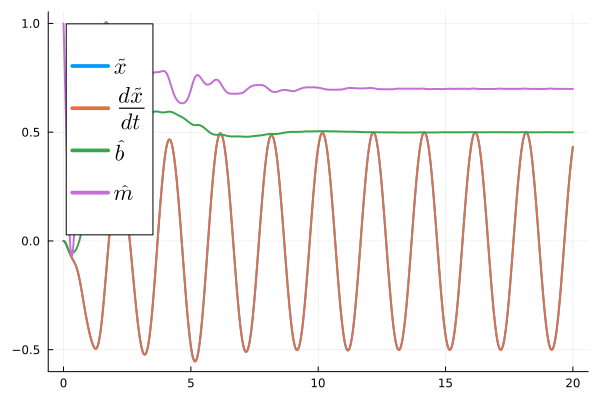
\includegraphics[width=0.5\textwidth]{./figures/adaptationrule1.pdf}
  \caption{Simulation showing the convergence of the system state and parameter
  estimates.}
  \label{fig:adaptation}
\end{figure}

\begin{figure}[b!]
  \centering
  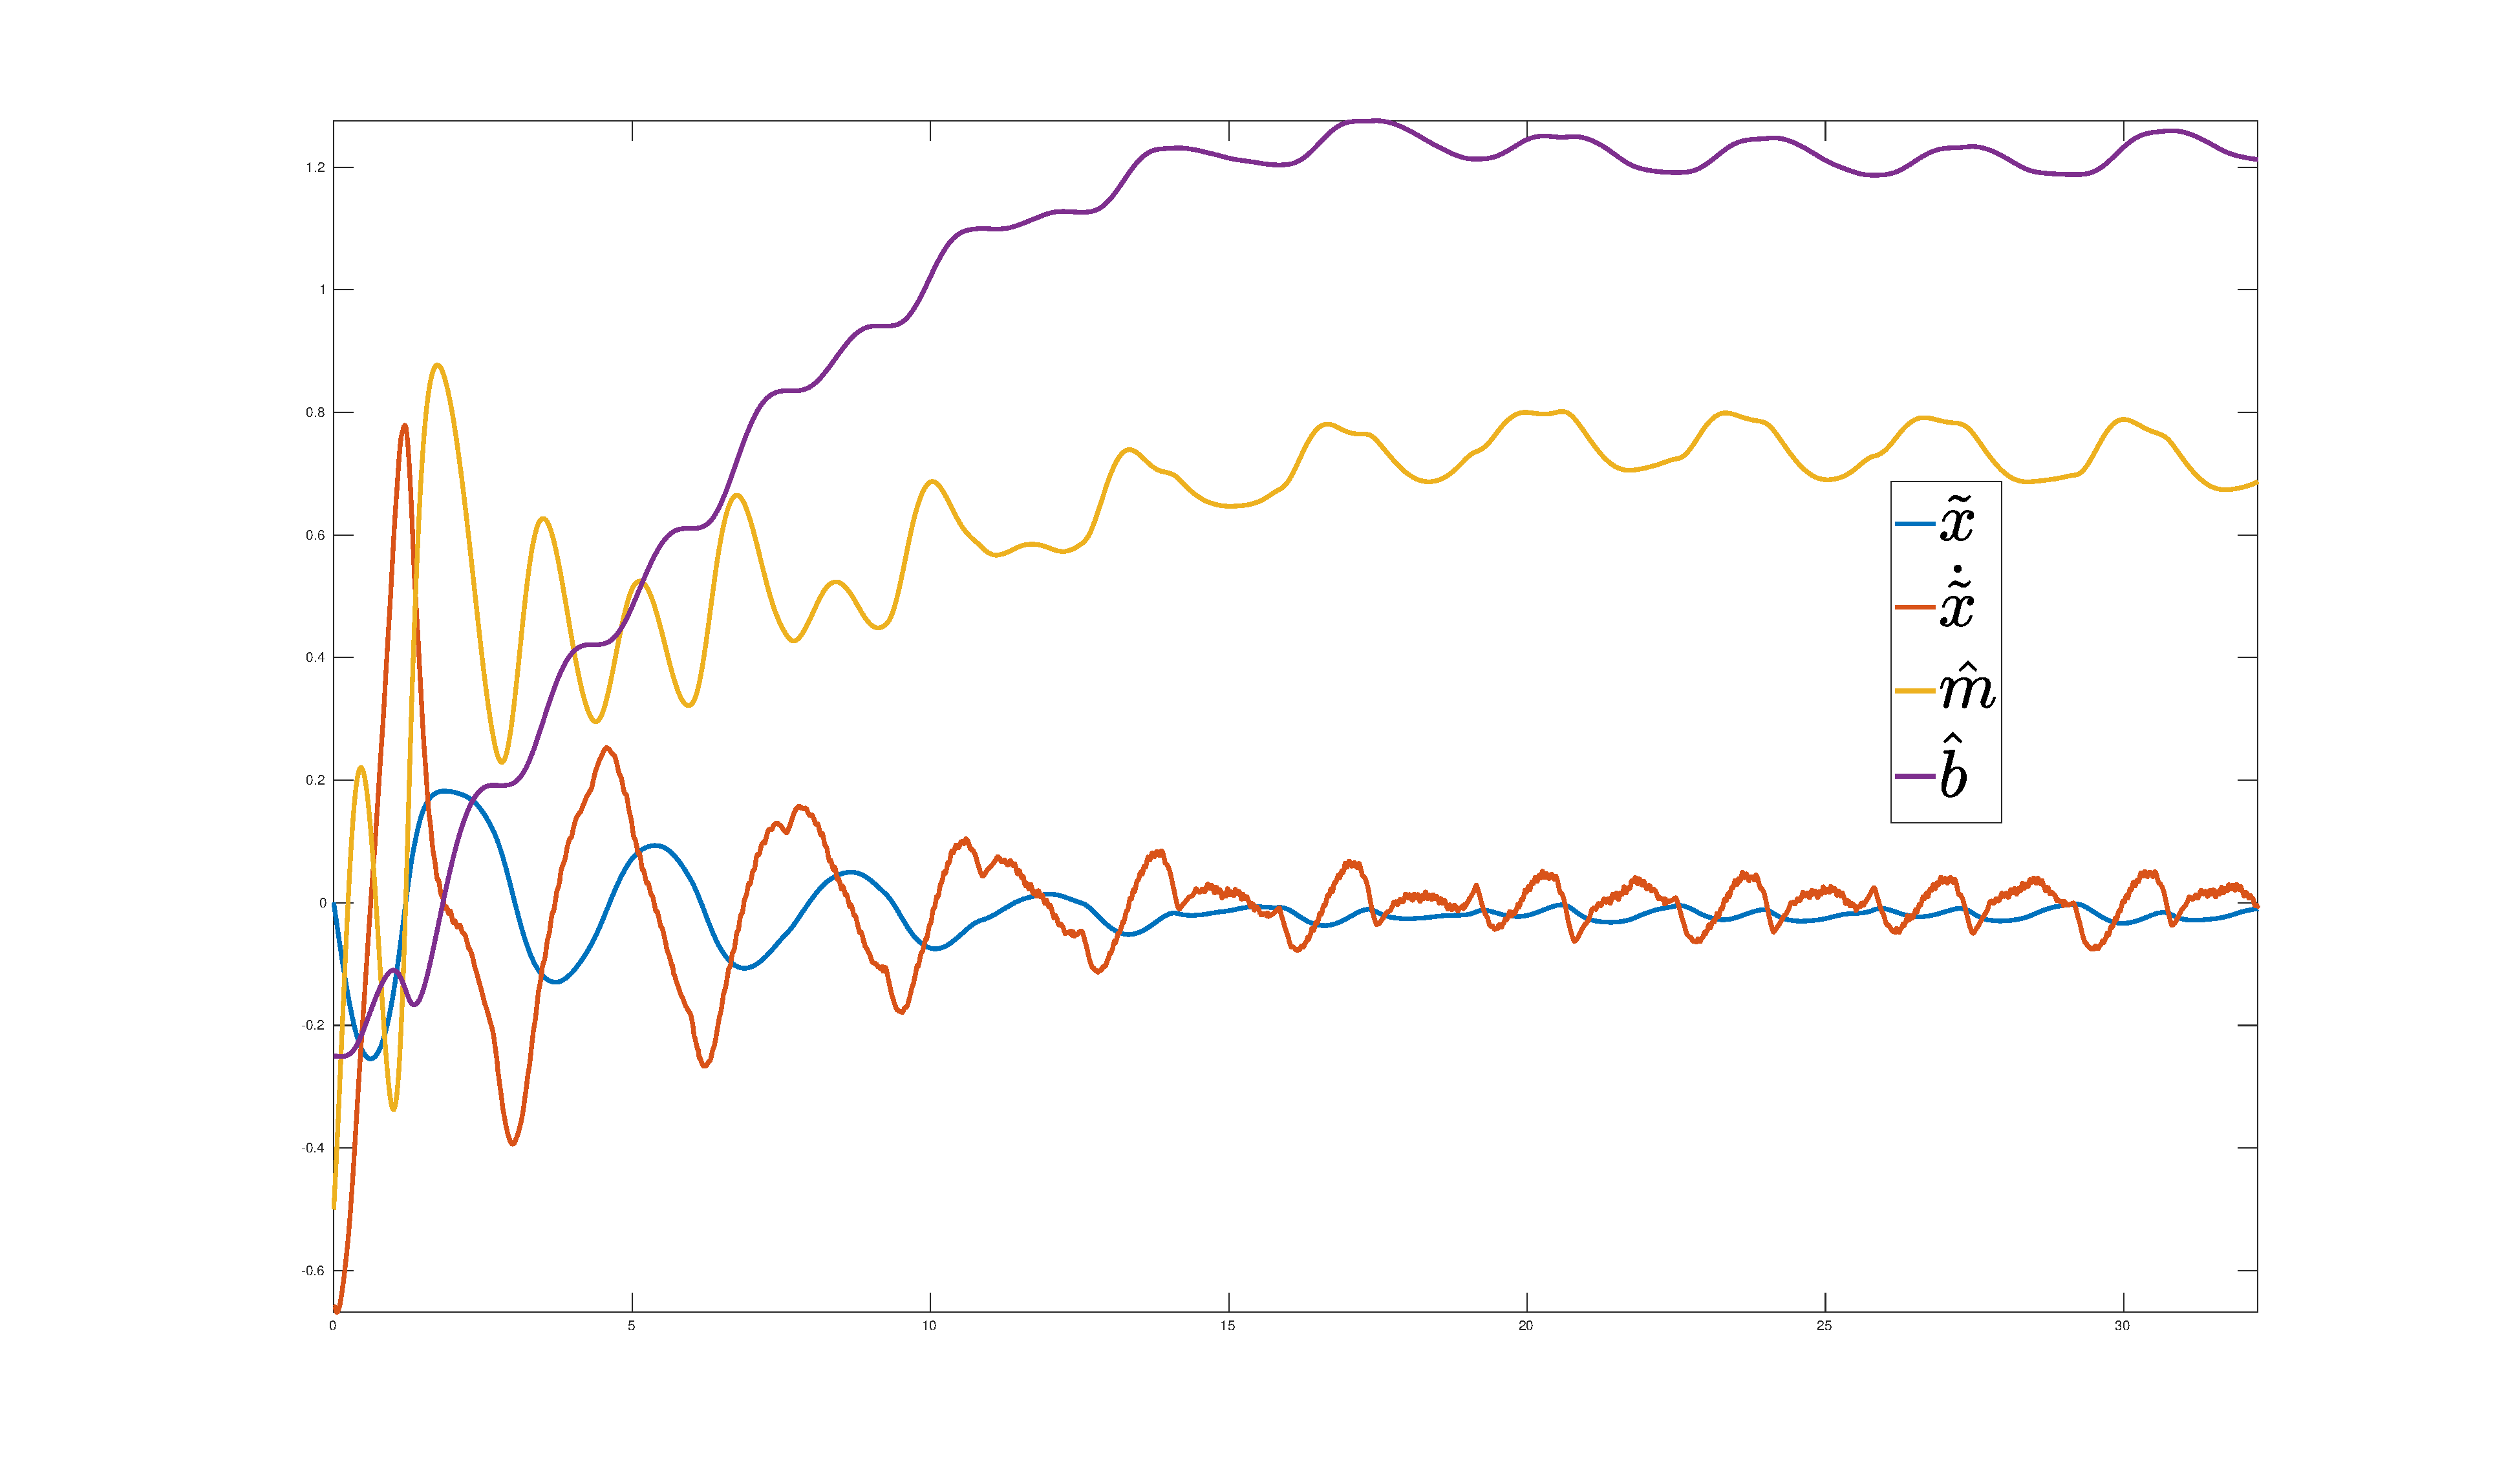
\includegraphics[width=0.5\textwidth]{./figures/station2_adaptation.eps}
  \caption{Hardware implementation of the estimation algorithm.}
  \label{fig:hardware}
\end{figure}

In Figure~\ref{fig:adaptation}, we plot the response of the system to the
control and adaptation laws~(\ref{eq:controller}, \ref{eq:adaptation}),
implemented in simulation. The constants that are used are as follows: $(A,
\omega, \varphi) = (\nicefrac{3}{10}, \nicefrac{3\pi}{5}, 0^\circ)$ and $(k,
\lambda) = (1, 4)$. The real mass and damping of the system is $(m, b) = (0.75,
1.22)$ and their estimates start at $(\hat{m}, \hat{b}) = (-\nicefrac{1}{2},
-\nicefrac{1}{4})$.

In Figure~\ref{fig:hardware}, we plot the response of the system to the control
and adaptation laws ~(\ref{eq:controller}, \ref{eq:adaptation}), implemented on
a real cart system. The constants used are as follows: $(A, \omega, \varphi) =
(\nicefrac{3}{10}, \nicefrac{3\pi}{5}, 0^\circ)$ and $(k, \lambda) = (1, 4)$. We
did not know the real mass and damping of the system and set our initial guesses
of them to be $(\hat{m}, \hat{b}) = (-\nicefrac{1}{2}, -\nicefrac{1}{4})$.


\section{Conclusion}
\label{sec:conclusion}

We have shown that our estimation algorithm for the linear second-order
mechanical system guides the estimates of the mass and the damping coefficient
to tend to their correct values.


\bibliographystyle{ieeetr}        
\bibliography{bib/references.bib}  

% \input{contents/appendix.tex}
% 
% \vspace{9em}
% 
% \begin{IEEEbiography}[{\includegraphics[width=1in,height=1.25in,clip,keepaspectratio]{siric.jpg}}]
%     %
%     {Wankun Sirichotiyakul} (M'21) was born in Bangkok, Thailand. He received
%     the B.Sc. (2017) and M.Sc. (2019) degrees in mechanical engineering from
%     Boise State University, Boise, Idaho, USA, where he is currently working
%     toward the Ph.D. degree in electrical and computer engineering. 
%     
%     His research interests are in the intersection of optimization and machine
%     learning approaches to the control of robotic systems.
% \end{IEEEbiography}
% 
% \begin{IEEEbiography}[{\includegraphics[width=1in,height=1.25in,clip,keepaspectratio]{ashen.jpg}}]
%     %
%     {Nardos A. Ashenafi} (M'21) was born and raised in Ethiopia. She came to the
%     United States to further her education in the field of engineering,
%     robotics, and control. She received the B.Sc degree in mechanical
%     engineering (2019) and the M.Engr degree in electrical engineering (2021)
%     from Boise State University, Idaho, USA. She is currently pursuing the Ph.D.
%     degree in electrical and computer engineering at Boise State University with
%     emphasis in robotics and control of dynamical systems. 
%     
%     Her interests include mechanical design, nonlinear
%     control, machine learning and mechatronics.
% \end{IEEEbiography}
% 
% \begin{IEEEbiography}[{\includegraphics[width=1in,height=1.25in,clip,keepaspectratio]{satic.jpg}}]
%     %
%     {AYKUT C. SATICI} (M'12) received the B.Sc. and M.Sc. degrees in
%     mechatronics engineering from Sabanci University, Istanbul, Turkey, in
%     2008 and 2010, respectively, and the Master's degree in mathematics from
%     the University of Texas, Dallas, TX, USA, in 2013. He received his Ph.D.
%     degree from the Electrical Engineering Department, University of Texas at
%     Dallas. 
% 
%     He is currently with the Boise State University where he is an assistant
%     professor of Mechanical and Biomedical Engineering. He has authored or
%     co-authored more than 30 technical papers in control and robotics. His
%     current research interests include robotics, geometric mechanics,
%     nonlinear control theory, and machine learning for robotics.
%     
%     Dr. Satici has been serving an Associate Editor for the International
%     Conference on Robotics and Automation for 3 years and is in the Program
%     Committee for American Control Conference 2023.
% \end{IEEEbiography}
% 
% \vspace{20.5em}

\end{document}
